\documentclass{article}
\usepackage{tikz}
\usepackage{pdflscape}
\usetikzlibrary{calc,positioning,shapes.geometric,arrows.meta}

\makeatletter
\pgfdeclareshape{satnode}{
\inheritsavedanchors[from={rectangle}]
\inheritbackgroundpath[from={rectangle}]
\inheritanchorborder[from={rectangle}]
\foreach \x in {center,north east,north west,north,south,south east,south west, east, west}{
\inheritanchor[from={rectangle}]{\x}
}
\foregroundpath{
\pgfpointdiff{\northeast}{\southwest}
\pgf@xa=\pgf@x \pgf@ya=\pgf@y
\northeast
\pgfpathmoveto{\pgfpoint{0}{0.45\pgf@ya}}
\pgfpathlineto{\pgfpoint{0}{-0.45\pgf@ya}}
\pgfpathmoveto{\pgfpoint{0.45\pgf@xa}{0}}
\pgfpathlineto{\pgfpoint{-0.45\pgf@xa}{0}}
\pgfpathmoveto{\pgfpointadd{\southwest}{\pgfpoint{-0.2\pgf@xa}{-0.3\pgf@ya}}}
\pgfpathlineto{\pgfpointadd{\southwest}{\pgfpoint{-0.5\pgf@xa}{-0.3\pgf@ya}}}
\pgfpathlineto{\pgfpointadd{\northeast}{\pgfpoint{-0.5\pgf@xa}{-0.3\pgf@ya}}}
\pgfpathlineto{\pgfpointadd{\northeast}{\pgfpoint{-0.2\pgf@xa}{-0.3\pgf@ya}}}
\pgfusepath{stroke}
}
}

\pgfdeclareshape{shpnode}
{
\inheritsavedanchors[from={rectangle}]
\inheritbackgroundpath[from={rectangle}]
\inheritanchorborder[from={rectangle}]
\foreach \x in {center,north east,north west,north,south,south east,south west,east,west}
{
\inheritanchor[from={rectangle}]{\x}
}
\foregroundpath
{
\pgfpointdiff{\northeast}{\southwest}
\pgf@xa=\pgf@x \pgf@ya=\pgf@y
\northeast
\pgfpathmoveto{\pgfpoint{0}{0.45\pgf@ya}}
\pgfpathlineto{\pgfpoint{0}{-0.45\pgf@ya}}
\pgfpathmoveto{\pgfpoint{0.45\pgf@xa}{0}}
\pgfpathlineto{\pgfpoint{-0.45\pgf@xa}{0}}
\pgfpathmoveto{\pgfpointadd{\southwest}{\pgfpoint{-0.5\pgf@xa}{-0.3\pgf@ya}}}
\pgfpathlineto{\pgfpointadd{\northeast}{\pgfpoint{-0.5\pgf@xa}{-0.3\pgf@ya}}}
\pgfusepath{stroke}
}
}
\makeatother



\begin{document}
\begin{landscape}
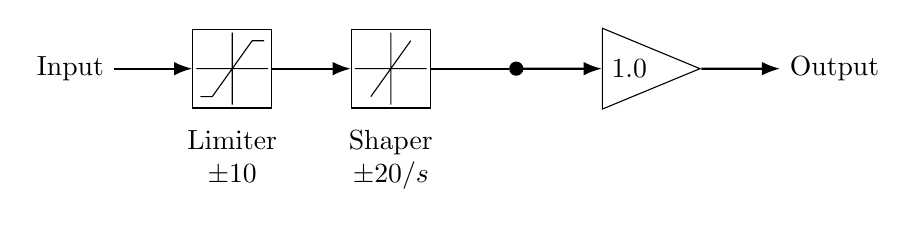
\begin{tikzpicture}
[Gain/.style={isosceles triangle, draw=black},
Junction/.style={circle, draw=black,fill=black,scale=0.5},
>=Latex];
\node[](Input)[]{Input};
\node[satnode,minimum size=1cm,draw](Lim1)[right=of Input]{};
\node[]()[below=1mm of Lim1]{\begin{tabular}{c}Limiter \\ $\pm10$ \end{tabular}};
\node[shpnode,minimum size=1cm,draw](Shp1)[right=of Lim1]{};
\node[]()[below=1mm of Shp1]{\begin{tabular}{c}Shaper \\ $\pm20/s$ \end{tabular}};
\node[Junction](J1)[right=of Shp1]{};
\node[Gain](Gain1)[right=of J1]{1.0};
\node[](Output)[right=of Gain1]{Output};
\draw[->,thick] (Input) -- (Lim1) ;
\draw[->,thick]  (Lim1) -- (Shp1);
\draw[-,thick]  (Shp1) -- (J1);
\draw[->,thick]  (J1) --(Gain1);
\draw[->,thick]  (Gain1) -- (Output);
\end{tikzpicture}
\end{landscape}
\end{document}

